Using our knowledge of geometric transformations and projective geometries, we can build up a model of a camera step by step. We standardize our reference frame by having the $z$ direction along the focal direction of the camera, the $x$ direction to the right, and the $y$ direction such that the right-hand rule is maintained. The origin is at the center of the camera.

We will describe the object of interest as a collection of points, $\mathbf{p} =  [x_i, y_i, z_i, 1] \text{ for } i = 1,2,\cdots,N$. For a complete picture, any given operation will be performed on all points. For simplicity, the following equations will demonstrate the process on a single point of the object.

First, we need to describe the location and orientation of the object with respect to the camera. This can be done with a 3D homogeneous transformation matrix (translation and rotation) (Eq. \ref{eq:4x4-homog-transformation}).

\begin{equation}
    \tilde{\mathbf{p}}' = \begin{bmatrix}
        R_{3 \times 3} & \mathbf{t}_{3 \times 1} \\ \mathbf{0}_{1 \times 3} & 1
    \end{bmatrix} \tilde{\mathbf{p}}
    \label{eq:4x4-homog-transformation}
\end{equation}

Then, we use a projective transformation that determines the perspective scaling between the objects actual location and the image place at the focal distance. Geometrically, this relationship can be visualized with similar triangles (Fig. \ref{fig:perspective-projection}), and quantified using the ratio of lengths (Eq. \ref{eq:perspective-projection}). In these equations, $f'$ is the focal distance in units of length.

\begin{figure}[h!]
    \begin{center}
        \includegraphics[width=0.85\linewidth]{figs/background/png/perspective-projection.png}
    \end{center}
    \caption{The geometry of perspective projection can be visualized by using similar triangles. The overall scaling of the image is based on the ratio of the focal length to the depth of the object.}
    \label{fig:perspective-projection}
\end{figure}


\begin{equation}
    \begin{aligned}
        \tilde{\mathbf{x}}_{i} &= \begin{bmatrix}
            f' & 0 & 0 \\ 0 & f' & 0 \\ 0 & 0 & 1 
        \end{bmatrix} \tilde{\mathbf{p}}' \\
        &\text{where} \\
        x_i &= p_x'\frac{f'}{p_z'} \\
        y_i &= p_y'\frac{f'}{p_z'} \\
    \end{aligned}
    \label{eq:perspective-projection}
\end{equation}

We can account for any image offset using the principal point. This is the point where the ray from the x-ray to the image plane is perpendicular, which is typically near the center of the image, though not always.

\begin{equation}
    \begin{aligned}
        \tilde{\mathbf{x}}_{i} &= \begin{bmatrix}
            f' & 0 & c_x \\ 0 & f' & c_y \\ 0 & 0 & 1 
        \end{bmatrix} \tilde{\mathbf{p}}' \\
        &\text{where} \\
        c_x &\approx \frac{W_{image}}{2} \\
        c_y &\approx \frac{H_{image}}{2} \\
    \end{aligned}
    \label{eq:perspective-projection}
\end{equation}

Lastly, we need to convert the points in $\tilde{\mathbf{x}}_i$ to pixel coordinates using the pixel scale factor, $k_x,k_y$ for the x and y factors, respectively.

\begin{equation}
    \begin{aligned}
        \tilde{\mathbf{x}}_{pix} &= \begin{bmatrix}
            k_x & 0& 0 \\ 0 & k_y & 0 \\ 0 & 0 & 1
        \end{bmatrix} \begin{bmatrix}
            f' & 0 & c_x \\ 0 & f' & c_y \\ 0 & 0 & 1 
        \end{bmatrix} \\
        & = \begin{bmatrix}
            f_x & 0 & c_x \\ 0 & f_y & c_y \\ 0 & 0 & 1 
        \end{bmatrix}\\
        &\text{where}\\
        f_x &= k_x f' \text{        and        } f_y = k_y f' \\
        &\text{Are focal distances in units of pixels} 
    \end{aligned}
\end{equation}